\documentclass[10pt, conference, compsocconf]{IEEEtran}
% \documentclass[runningheads]{includes/llncs}
% \documentclass[final,a4paper,12pt,english]{includes/llncs}
\usepackage{fancyvrb}
\usepackage{academicons}
\newcommand{\orcid}[1]{\href{https://orcid.org/#1}{\textcolor[HTML]{A6CE39}{\aiOrcid}}}
\newcommand*{\doi}[1]{\href{http://dx.doi.org/#1}{doi: #1}}


\usepackage{alltt, amsmath, amssymb, amsfonts, array}
\usepackage{cite}
\usepackage{enumerate}
\usepackage[T1]{fontenc} %%%key to get copy and paste for the code!
\usepackage[utf8]{inputenc} %%% to support copy and paste with accents for frnehc stuff
\usepackage[scaled=0.85]{helvet}
\usepackage{graphicx}
\usepackage{ifthen}
\usepackage{latexsym}
\usepackage{url}            
\usepackage{xcolor, xspace}
\usepackage{stmaryrd}
\usepackage{times}
\usepackage{wrapfig}
\usepackage[inline]{enumitem}  
\usepackage{hyperref}
\usepackage{array}
\usepackage{booktabs, multirow} % for borders and merged ranges
\usepackage{changepage}
\usepackage[english]{babel}
\usepackage{graphicx}
\usepackage{ifdraft}
\usepackage[utf8]{inputenc}
\usepackage{lipsum, listings}    
\usepackage{newunicodechar}
\usepackage[square,sort,comma,numbers]{natbib}
\usepackage{xspace}     
\usepackage{textcomp, threeparttable}
\usepackage{pifont}
\usepackage{soul}% for underlines
\usepackage[inline]{enumitem}
\usepackage{subfig}
\usepackage{numprint}
\usepackage{hyperref}
% \usepackage[colorlinks=true,linkcolor=black,anchorcolor=black,citecolor=black,filecolor=black,menucolor=black,runcolor=black,urlcolor=black]{hyperref}
\usepackage{lineno}
\usepackage[font=small,labelfont=bf]{caption}

\usepackage{amsmath, amssymb, array}
\usepackage{booktabs, multirow} % for borders and merged ranges
\usepackage{changepage}
\usepackage[english]{babel}
\usepackage{graphicx}
\usepackage{ifdraft}
\usepackage[utf8]{inputenc}
\usepackage{lipsum, listings}    
\usepackage{natbib, newunicodechar}
\usepackage{xspace}     
\usepackage{textcomp, threeparttable}
\usepackage{pifont}
\usepackage{color, colortbl}
\usepackage{soul}% for underlines
% \usepackage[table]{xcolor} % for cell colors
% \usepackage[colorlinks=true,linkcolor=black,anchorcolor=black,citecolor=black,filecolor=black,menucolor=black,runcolor=black,urlcolor=black]{hyperref}
% \usepackage{lineno}
%\linenumbers

\newunicodechar{✓}{\ding{51}}
\newunicodechar{✗}{\ding{55}}

% \theoremstyle{definition}
% \newtheorem{definition}{Definition}[section]
% \theoremstyle{remark}
% \newtheorem*{remark}{Remark}

\newcolumntype{L}{>{\centering\arraybackslash}m{2cm}}
\newcolumntype{B}{>{\arraybackslash}p{0.5\textwidth}}
\newcolumntype{S}{>{\centering\arraybackslash}m{.5cm}}

\definecolor{ivory}{rgb}{1.0, 1.0, 0.94}
\definecolor{lightgray}{rgb}{0.88,1,1}

\newcommand{\dquotes}[1]{``#1''}
\newcommand{\nnbb}[2]{
    \fbox{\bfseries\sffamily\scriptsize#1}
    {\sf\small$\blacktriangleright$\textit{#2}$\blacktriangleleft$}
}
\newcommand{\ap}[1]{\nnbb{\textcolor{blue}{Ant}}{\textcolor{blue}{#1}\xspace}}
\newcommand{\Oracle}[0]{Gas Oracle\xspace}
\newcommand{\Oracles}[0]{Gas Oracles\xspace}
\newcommand{\miro}[0]{Mir{\'{o}}\xspace}
\newcommand{\gr}{graphical representation\xspace}
\newcommand{\M}{Miró\xspace}

% Define a custom color scheme
\definecolor{codebackground}{rgb}{0.75,0.99,0.99} % Light gray background
\definecolor{codecomment}{rgb}{0.5,0.5,0.5}       % Gray for comments
\definecolor{codekeyword}{rgb}{0,0,1}             % Blue for keywords
\definecolor{codestring}{rgb}{0.56,0,0.1}         % Dark red for strings

% Python code style configuration
\lstdefinestyle{inferno}{
    backgroundcolor=\color{codebackground}, % Background color
    commentstyle=\color{codecomment},       % Comment style
    keywordstyle=\color{codekeyword},       % Keyword style
    stringstyle=\color{codestring},         % String style
    basicstyle=\ttfamily\small,             % Font and size
    breaklines=true,                        % Automatic line breaking
    numbers=none,                           % No line numbers
    frame=single,                           % Single-line frame
    rulecolor=\color{gray},                 % Border color
    showspaces=false,                       % Hide spaces
    showstringspaces=false,                 % Hide spaces in strings
    showtabs=false,                         % Hide tabs
    tabsize=4,                              % Tab width
    language=Python                         % Specify Python as the language
}


\begin{document}
% https://easychair.org/cfp/DLT-2022
% \title{A comparison between \\Libra/Diem and other Blockchains}
% \title{Comparative Study on Libra, Ethereum and Solana Blockchain}
\title{A Study on \dots}

\author{
    \IEEEauthorblockN{Giuseppe Antonio Pierro}
    \IEEEauthorblockA{
        \textit{Dep. of Mathematics and Computer Science} \\
        \textit{University of Cagliari}\\
        Cagliari, Italy\\
        antonio.pierro@gmail.com
    }
}
\maketitle

% The Libra Blockchain, 2020-05-26.pdf

\begin{abstract}
% TODO the abstract should be shorter
This research paper aims to analyze the Airbnb dataset, focusing on various factors that influence prices of listings. 
The dataset encompasses key features such as price, room type, person capacity, host characteristics, cleanliness rating, and geographical attributes. 
The study poses the research question: "What are the factors that influence the price and location of Airbnb listings?" 
The author postulates that the pricing is significantly influenced by the distance from the center.

\lipsum[1]
\end{abstract}

\begin{IEEEkeywords}
Airbnb, location price, geographical attribute
\end{IEEEkeywords}

%:================================
\section{Introduction}
The rise of Airbnb~\cite{andreu2020airbnb} has transformed the hospitality industry, allowing individuals to rent accommodations. 
Understanding the determinants of pricing and location is crucial for both hosts and guests. 
This paper explores the dataset to uncover insights into the factors shaping Airbnb prices and locations.

\lipsum[2-3]

\lipsum[3-4]

\lipsum[5-6]

\section{Dataset Description}
The Airbnb dataset consists of several columns, including price, room type, person capacity, host characteristics, cleanliness rating, and geographical attributes \cite{bathwal2024flightprice}. 
These variables provide a comprehensive view of the listings and their characteristics.

The mean, the median, minimum (min), the 25th, 50th, and 75th percentiles and maximum (max) are calculated for each variable shown in the table.

\begin{table*}[!htp]
  \centering
  \caption{Generated by Spread-LaTeX}\label{tab:spread_latex}
  \resizebox{\textwidth}{!}{%
  \begin{tabular}{p{0.2\textwidth}p{0.8\textwidth}}
  \toprule
  \textbf{Name} & \textbf{Description} \\
  \midrule
  realSum & Represents the total price or sum associated with the Airbnb listing. \\
  room\_type & Indicates the type of room, such as "Entire home/apt" or "Private room." \\
  room\_shared & Binary indicator (True/False) if the room is shared. \\
  room\_private & Binary indicator (True/False) if the room is private. \\
  person\_capacity & Specifies the maximum number of people the accommodation can host. \\
  host\_is\_superhost & Binary indicator (True/False) if the host is recognized as a superhost. \\
  multi & Binary indicator (True/False) if the listing is part of a multi-listing. \\
  biz & Binary indicator (True/False) if the listing is associated with a business. \\
  cleanliness\_rating & Represents the cleanliness rating of the accommodation. \\
  guest\_satisfaction\_overall & Represents the overall guest satisfaction rating. \\
  bedrooms & Specifies the number of bedrooms in the accommodation. \\
  dist & Represents the distance to a certain location or point of interest. \\
  metro\_dist & Represents the distance to a metro or subway station. \\
  attr\_index & Represents an attraction index, possibly related to nearby attractions. \\
  attr\_index\_norm & Normalized version of the attraction index. \\
  rest\_index & Represents a restaurant index, possibly related to nearby restaurants. \\
  rest\_index\_norm & Normalized version of the restaurant index. \\
  lng & Represents the longitude coordinate of the accommodation. \\
  lat & Represents the latitude coordinate of the accommodation. \\
  \bottomrule
  \end{tabular}%
  }
\end{table*}
  
\lipsum[1]




\lipsum[2-3]

\section{Research Questions}
The primary research question addressed in this study is: "What are the factors that influence the price and location of Airbnb listings?" 
This overarching question will guide the exploration of various aspects within the dataset.

\lipsum[2]

This study aims to explore the patterns and relationships within the Los Angeles Airbnb dataset. Specifically, it seeks to address the following research questions:
\begin{itemize}
    \item \textbf{RQ\_1}: What patterns exist in the data regarding property types, pricing, and availability across different neighborhoods in Los Angeles?
    \item \textbf{RQ\_2}: How do key variables such as price and property location interact to influence occupancy rates?
    \item \textbf{RQ\_3}: What factors most significantly impact customer ratings and reviews, and how do they correlate with host behavior or property characteristics?
\end{itemize}

\lipsum[3]

\section{Research Hypotheses}
Based on initial observations, a hypothesis is proposed that the distance from the city center significantly influences Airbnb pricing. 
It is hypothesized that listings closer to the center command higher prices due to factors such as proximity to attractions, events, and better infrastructure.

\begin{itemize}
  \item \textbf{RH\_1\_0}: There are no significant patterns in the data regarding property types, pricing, and availability across different neighborhoods in Los Angeles.  
  \item \textbf{RH\_1\_A}: Significant patterns exist in the data regarding property types, pricing, and availability across different neighborhoods in Los Angeles.  

  \item \textbf{RH\_2\_0}: There is no significant interaction between key variables such as price and property location in influencing occupancy rates.  
  \item \textbf{RH\_2\_A}: Key variables such as price and property location significantly interact to influence occupancy rates.  

  \item \textbf{RH\_3\_0}: Factors such as customer ratings and reviews are not significantly correlated with host behavior or property characteristics.  
  \item \textbf{RH\_3\_A}: Factors such as customer ratings and reviews are significantly correlated with host behavior or property characteristics.  
\end{itemize}

\lipsum[2-3]

\section{Results}
\lipsum[2-3]
Table~\ref{tab:df-statitistics} shows the summary statiticst of Airbnb dataset. 
\begin{figure}[ht]
  \centering
  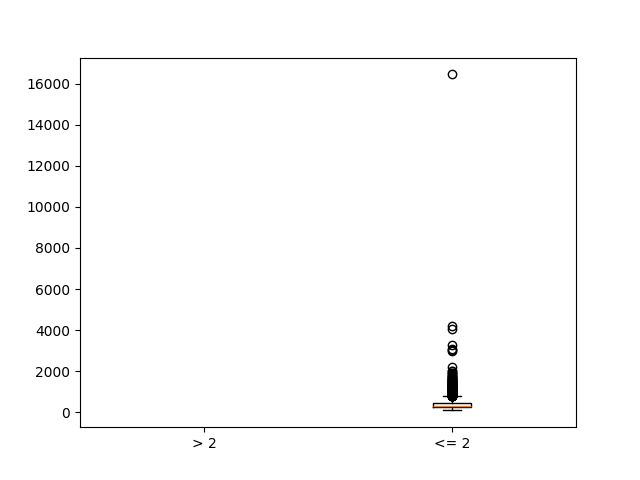
\includegraphics[width=\columnwidth]{figures/price-vs-distance-paris.png}
  \caption{Box plot representing the price based on the distance from the metro for the city of Paris}
  \label{fig:box-plot-paris}
\end{figure}
\lipsum[1]

Figure \ref{fig:fig2} \lipsum[1]

\begin{table}[ht]
  \caption{Summaries of the Airbnb data-set}
  \centering
  \resizebox{\columnwidth}{!}{%
  \begin{tabular}{rlllll}
    \hline
    & file size (B) & gas\_used & bytesLength & scriptBytesLength & TPS \\ 
    \hline
    Min.     & 370.0   & 74.00   & 834   & 526.0  & 0.00 \\ 
    1st Qu.  & 606.0   & 74.00   & 1066  & 758.0  & 48.00 \\ 
    Median   & 606.0   & 74.00   & 1066  & 758.0  & 60.00 \\ 
    Mean     & 605.2   & 77.81   & 1065  & 757.2  & 62.45 \\ 
    3rd Qu.  & 606.0   & 74.00   & 1066  & 758.0  & 80.00 \\ 
    Max.     & 606.0   & 1748.00 & 1066  & 758.0  & 180.00 \\ 
    \hline
  \end{tabular}%
  }
  \label{tab:df-statitistics}   
\end{table}

\begin{figure*}[ht]
  \centering
  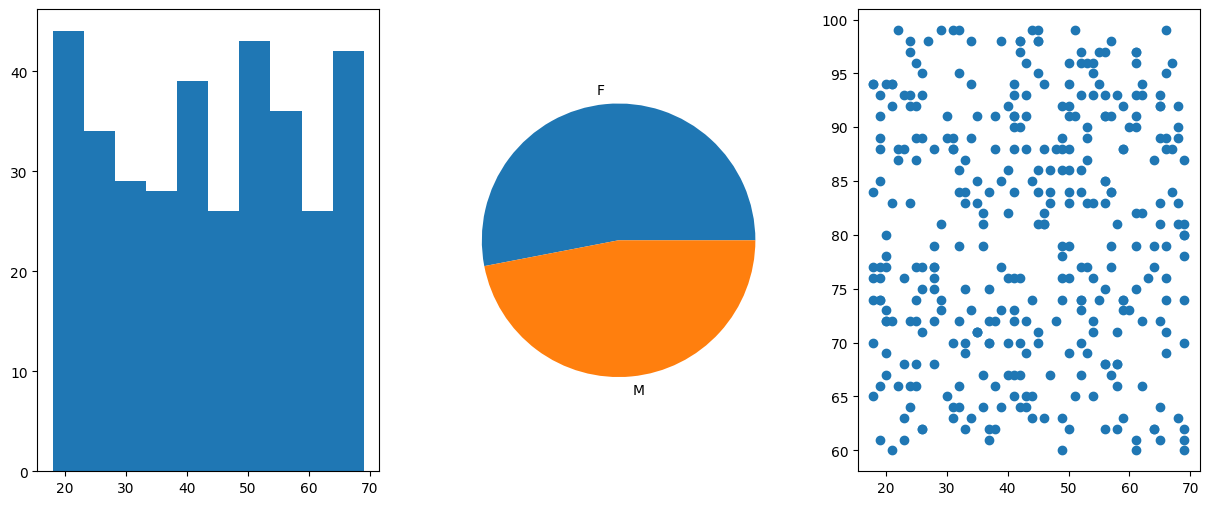
\includegraphics[width=.99\textwidth]{figures/subplot.png}
  \caption{\lipsum[1]}
  \label{fig:fig2}
\end{figure*}
\lipsum[1]

Figure \ref{fig:heat-map} \lipsum[1]
\begin{figure}[ht]
  \centering
  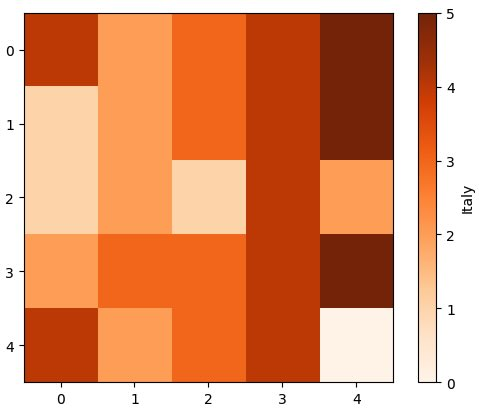
\includegraphics[width=\columnwidth]{figures/heat-map.jpg}
  \caption{Box plot representing the price based on the distance from the metro for the city of Paris}
  \label{fig:heat-map}
\end{figure}

\section{Discussion}
The discussion section will delve into the findings related to the research questions and hypotheses. 
It will explore the correlation between distance from the center and pricing, considering potential confounding variables. 
Additionally, it will analyze how other variables such as room type, host superhost status, and cleanliness rating impact pricing and location.

\lipsum[1]

\lipsum[2]

\lipsum[3-4]

\section{Conclusion}
In conclusion, this research contributes valuable insights into the factors influencing Airbnb prices and locations. 
The analysis sheds light on the importance of geographic proximity to the center and other variables in determining listing prices. 
These findings can benefit both hosts and guests in making informed decisions within the Airbnb marketplace.

This research provides a foundation for further exploration and understanding of the dynamic factors at play in the Airbnb ecosystem.

\lipsum[1]

\section{authors}
\subsection{Giuseppe Antonio Pierro}
Giuseppe Antonio Pierro obtained his Ph.D. in Physics from the University of Bari and CERN, Geneva~\cite{cern},
and his Ph.D. in Mathematics and Computer Science from the University of Cagliari and Inria, Lille. 
Prior to that, \lipsum[1]

\section{Appendix}

The analysis on the dataset was conducted using the Python programming language~\cite{rayhanrise, van1995python} and some of its libraries. 
The Python libraries utilized include matplotlib~\cite{Hunter:2007}, pandas, and numpy.

\lipsum[2-3]

Listing \ref{mylist2} \dots.

\begin{lstlisting}[style=inferno, label={mylist2}, caption={Recursive Factorial Function}, linewidth=\columnwidth]
  # This is a sample Python code
  def greet(name):
      """Function to greet a user"""
      print(f"Hello, {name}!")
  
  names = ["Alice", "Bob", "Charlie"]
  for name in names:
      greet(name)
\end{lstlisting}

\lipsum[4]
  

Listing \ref{mylist3} \lipsum[1]
\begin{lstlisting}[style=inferno , label={mylist3}, caption={Recursive Factorial Function}, linewidth=\columnwidth] 
import kagglehub

# Download latest version
path = kagglehub.dataset_download("ziya07/community-health-evaluation-dataset")

print("Path to dataset files:", path)
import pandas as pd
df = pd.read_csv(path + '/community_health_evaluation_dataset.csv')
print(df.columns)
\end{lstlisting}


\bibliographystyle{IEEEtran}
\bibliography{bibliography/main}
\end{document}
